\documentclass[11pt]{article}
\usepackage[margin=1in]{geometry} 
\usepackage{amsmath,amsthm,amssymb,amsfonts}
\usepackage{graphicx}
\usepackage{biblatex}
\newcommand{\N}{\mathbb{N}}
\newcommand{\Z}{\mathbb{Z}}
 
\newenvironment{problem}[2][Problem]{\begin{trivlist}
\item[\hskip \labelsep {\bfseries #1}\hskip \labelsep {\bfseries #2.}]}{\end{trivlist}}
 
\begin{document}
 
\title{Sudoku Solver \large  \\ CSE 841: Artificial Intelligence Final Project Writeup}
\author{Rundong Zhao}
\maketitle
 
\section {Abstract}
This project is for studying Constraint Satisfaction Problem (CSP). In general, CSP will include a set of \textbf{variables} within a certain domain and a set of \textbf{constraints}.  The goal is to find an \textbf{assignment} to the variables that can satisfy the set of constraints. This project focuses on Sudoku as a specific CSP problem. There are classic methods to deal with CSP, such as backtracking. [1] turns Sudoku to a Satisfiability Problem (SAT), which will try to use inference but not search. In this project, three algorithms are implemented, which are simple search without any heuristics, search with Minimum Remaining Value (MRV) heuristic and the SAT encoding. A wide range of Sudokus with different difficulty are tested and analyzed on the proposed algorithms. And the SAT transformation out-performs the other two algorithms significantly.

\section {Sudoku}
A Sudoku problem is represented by a $9 \times 9$ grid, which comprises nine $3 \times 3$ sub-grids. The objective is to fill the grid with digits from $1 - 9$ such that each column, each row and each of the $3 \times 3$ subgrids contain all the digits from $1 - 9$. A Sudoku will only admit exactly one solution, and all the hints will not contain any redundant information.

\section {Algorithms}
There are totally 3 algorithms that are implemented, which are simple search without any heuristics (SS), search with Minimum Remaining Value heuristics (SMRV) and the SAT encoding (SATE).

\subsection {Simple Search without any Heuristics}
SS algorithm is literally discribed by its name, it is very simple. The algorithm just scan the $9 \times 9$ grid from left to right, from top to bottom, until a blank is found. Then the contraints on row, column and block are applied to find the potential numbers that could be inserted at this blank. And basically, this just start several search branches based on the potential numbers. The algorithm will recursively construct and search through branches, and will terminate if a valid solution is found. 

\subsection {Search with Minimum Remaining Value Heuristic}
Similar to SS, SMRV also contruct and search through branches spaned by potential numbers in each blank. The only difference is that we will first use Minimum Remaining Value heuritic to decide which blank to start the search. Finally, the size of search tree will be minimal in a greedy way, which will drastically reduce the search time until a valid solution is found.

\subsection {SAT Encoding}
A SAT problem is another type of CSP. By resorting to SAT, we want to harness the inference techniques already developed in SAT to further reduce the search tree. This section will first address the basics of SAT, second introduce how to transform the Sudoku problem to SAT, and last SAT inference Techniques which will further improve the performance.

\subsubsection{Satisfiability}
A SAT problem is represented by $n$ propositional \textbf{variables} $x_1, x_2, ... , x_n$, which can be assigned as true or false. A \textbf{literal} $l$ is either a variable $x_i$ or its complement $\neg x_i$. We will use Conjunctive Normal Form (CNF) to address the SAT. a \textbf{clause} $\omega$ is a disjunction of literals and CNF formula $\varphi$ is a conjunction of clauses. A clause with a single literal is said to be \textit{unit} and its literals has to be assigned value 1 for the clause to be satisfied. The derivation of an \textit{empty} clause indicates that the formula is \textit{unsatisfied} for the given assignment. The formula is \textit{satisfied} if all its clauses are satisfied. The SAT is to decide whether there exists an assignment to the variables such that the formula is satisfied. 

\subsubsection{Sudoku to SAT Encoding}
A sudoku can be easily transformed into SAT, except that a siginificant number of variables and clauses are needed. We use $9 \times 9 \times 9 = 729$ propositional variables to encode Sudoku by SAT. For each entry of the $9 \ times 9$ grid, we associate $9$ variables. We use $s_{xyz}$ to represent the variables. Variable $s_{xyz}$ is assigned true if and only if the entry in row $x$ and column $y$ is assigned number $z$.

The encoding has four catogories, which are, first, there is at least one number in each entry; second, each number appears at most once in each row; third, each number appears at most once in each column; fourth, each number appears at most once in each $3 \times 3$ sub-grid. And the formulation are as follows:
\begin{itemize}
	\item There is at least one number in each entry: \\
		\begin{equation}
		\wedge_{x=1}^{9} \wedge_{y=1}^{9} \wedge_{z=1}^{9} s_{xyz}  \large
		\end{equation}
	
	\item Each number appears at most once in each row: \\
		\begin{equation}
		\wedge_{y=1}^{9} \wedge_{z=1}^{9} \wedge_{x=1}^{8} \wedge_{i=x+1}^{9} 
		\neg s_{xyz} \vee \neg s_{iyz} \large
		\end{equation}
		
	\item Each number appears at most once in each column: \\
		\begin{equation}
		\wedge_{x=1}^{9} \wedge_{z=1}^{9} \wedge_{y=1}^{8} \wedge_{i=y+1}^{9}
		\neg s_{xyz} \vee \neg s_{xiz}  \large
		\end{equation}
		
	\item Each number appears at most once in each $3 \times 3$ sub-grid: \\
		\begin{equation}
		\wedge_{z=1}^{9} \wedge_{i=0}^{2} \wedge_{j=0}^{2} \wedge_{x=1}^{3} \wedge_{y=1}^{3} \wedge_{k=y+1}^{3}
		\neg s_{(3i+x)(3j+y)z} \vee \neg s_{(3i+x)(3j+k)z} \large
		\end{equation}
		\begin{equation}
		\wedge_{z=1}^{9} \wedge_{i=0}^{2} \wedge_{j=0}^{2} \wedge_{x=1}^{3} \wedge_{y=1}^{3} 
		\wedge_{k=x+1}^{3} \wedge_{l=1}^{3}
		\neg s_{(3i+x)(3j+y)z} \vee \neg s_{(3i+k)(3j+l)z} \large
		\end{equation}
\end{itemize} 

In this encoding, the CNF formula have 8892 clauses, of which 81 clauses are 9-ary and the remaining 8748 clauses are binary.

\subsubsection{SAT Inference Techniques}
We will breifly review inference techniques for CNF formulas. We may derive additional information from the original formula, such as new simplified formula or determined assignment to certain variables.

One of the well-known inference techniques for SAT is \textit{resolution}. In general, 
\begin{equation}
(x_i \vee \alpha) \wedge (\neg x_i \vee \beta) \Rightarrow (\alpha \vee \beta)
\end{equation}
We will apply this rule for any pair of clauses containing $x$ and $\neg x$ to iteratively simplfy the CNF formula until a search bifurcation is inevitible. Two restricted forms of resolution, which are unit propagation and failed literal rule, are applied in the SAT solver in test.

\section {Data Set}
[2] provides a huge number of Sudoku problems. There are 5 groups, and each group contains 10000 Sudoku problems. The number of hints are 45, 40, 35, 30, 25 for different groups, representing the difficulty. And [3] also provide 10 evil Sudoku problems, which can clearly distinguish the performance of the proposed algorithms.

\section {Experiments Design}
By running proposed three algorithms on the wide range of testing sudoku problems, we will compare the efficiency of each algorithm. We will use histograms and line plots to illustrate the distribution of execution time on each group of data set. Part of the SAT solver code is borrowed from [4].

\section {Results}
We studied the results in several aspects.
\subsection{Execution Time Distribution}
Figure \ref{distribution} shows the distribution of execution time for different level of difficulty. Note that the difficulty is represented by number of hints given in each Sudoku. And we can see that, when the Sudoku problems are relatively easier (number of hints are 45, 40, 35), SS algorithm will beat the rest. But when the Sudoku probelms are relatively harder (number of hints are 30, 25), SAT algorithm will still remain a short execution time, but the search method will become worse.

\begin{figure}
\begin{center}
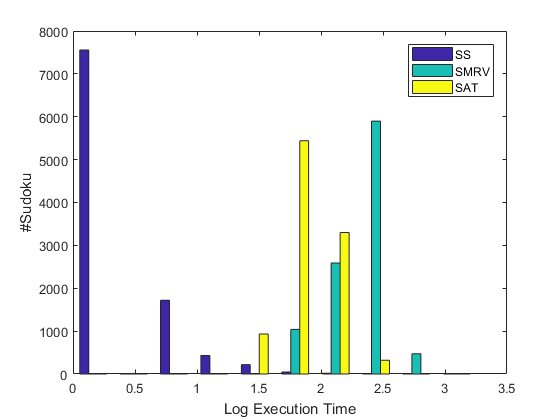
\includegraphics[width=0.49\textwidth]{fig/45Hints.png} 
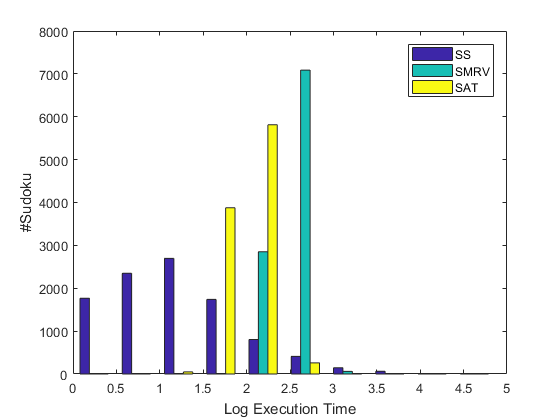
\includegraphics[width=0.49\textwidth]{fig/40Hints.png} 
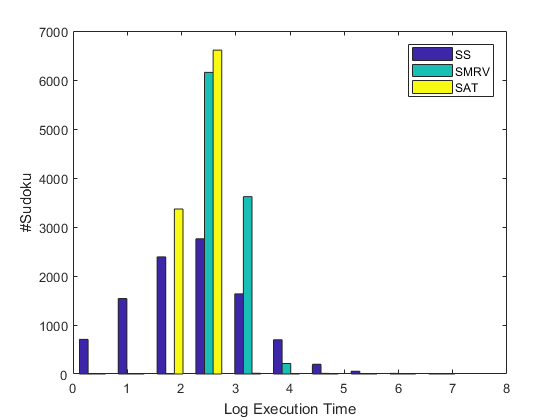
\includegraphics[width=0.49\textwidth]{fig/35Hints.png} 
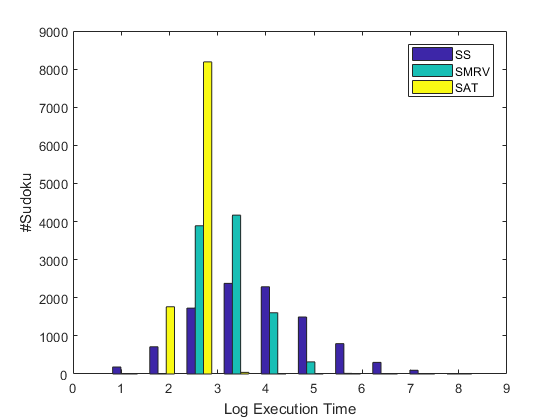
\includegraphics[width=0.49\textwidth]{fig/30Hints.png} 
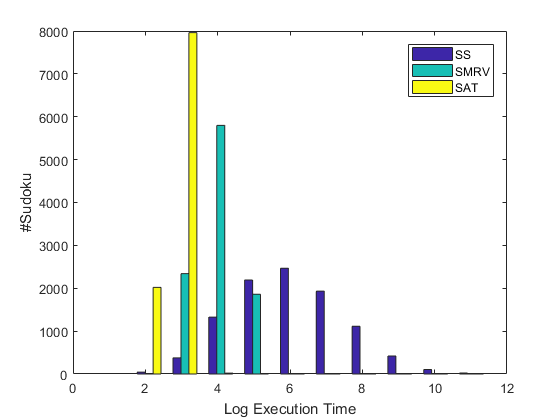
\includegraphics[width=0.49\textwidth]{fig/25Hints.png}
\end{center}

\caption{Here shows the distribution of log execution time for different levels of difficulty, with number of hints 45, 40, 35, 30, 25 respectively.}
\label{distribution}
\end{figure}

\subsection{Average Execution Time Plot}
Figure \ref{time} shows execution time plot for different levels of difficulty. And we can draw similar conclusions.

\begin{figure}
\begin{center}
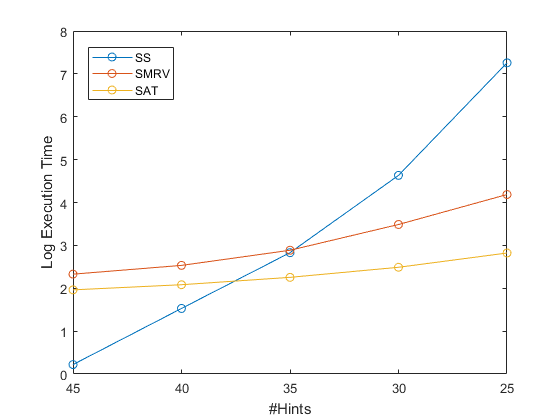
\includegraphics[width=0.58\textwidth]{fig/Time.png}
\end{center}

\caption{Here shows log execution time plot for different levels of difficulty.}
\label{time}
\end{figure}

\subsection{Performance on Challenges}
In order to further distinguish the proposed methods. We choose several evil difficulty Sudoku problems to show the power of SAT encoding. Figure \ref{evil} gives us 2 examples of evil difficulty Sudoku problems on which we test the proposed algorithms. With SAT encoding, the first Sudoku problem is solved in 130 milliseconds, and the second one is solved in 63 milliseconds. But the search algorithms can not reture a result within a reasonable amount of time (threshold is 100 seconds).

\begin{figure}
\begin{center}
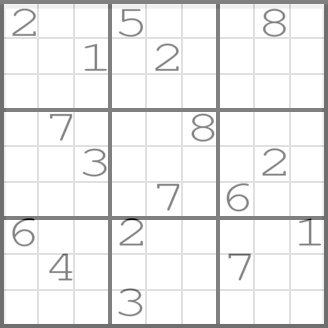
\includegraphics[width=0.4\textwidth]{fig/evil1.png}
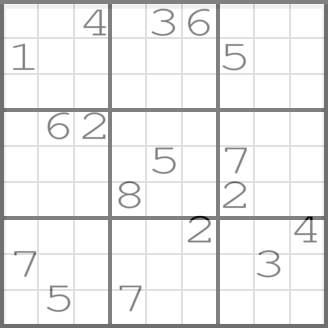
\includegraphics[width=0.4\textwidth]{fig/evil2.png}
\end{center}

\caption{Here shows 2 Sudoku problems with evil difficulty.}
\label{evil}
\end{figure}

\section {Conclusion}
We tested the proposed algorithms on 50000 standard testing cases, and several evil difficulty Sudoku problems.

We can see that by applying basic heuristic (MRV), the efficiency for relatively hard Sudoku problems has be improved in a logarithm level compared to simple search. The reason is that most of the time, by MRV heuristic, there is only 1 potential number for the targeted blank, meaning that we can avoid most of the searches. But for easy ones, the MRV procedure comprises a signigicant part of the total execution time, which causes the overhead.

We can see that SAT encoding has improve the efficiency much further compared with SMRV. For those evil level Sudoku problems, the search methods (SS, SMRV) even cannot give us results in a reasonable time. The SAT solver will try to expliot any clues by resolution to make inference. This way, most of the searches can be avoided to save a lot of execution time.

Finally, it is always recommended to use SAT encoding for Discrete Domain CSPs.

\section {Future Work}
There are several interesting ways to go. We can further investigate Sudoku problem, such as constructing hard Sudoku problems with 17 hints, extending 9 x 9 grid to n x n. We can also invesitage on applying SAT encoding to other Discrete Domain CPSs, to see how much the efficiency can be improved.

\begin{thebibliography}{9}

\bibitem{sudokuSat} 
Ines Lynce, Joel Ouaknine.
\textit{Sudoku as a SAT Problem}.
Proceedings of AIMATH, 2006.

\bibitem{source1}
\textit{http://www.printable-sudoku-puzzles.com/wfiles/}.
50000 Sudoku testing cases.

\bibitem{source2}
\textit{https://sites.google.com/site/hpenedones2/sourcecode/sudoku}.
Evil difficulty Sudoku testing cases.

\bibitem{togasat}
\textit{https://github.com/togatoga/togasat}.
Togasat SAT solver.
 
\end{thebibliography}

\end{document}